\section{Run-Time Assurance}

[DARREN - 1.5 pg]

Run-Time Assurance Architecture -- ASTM F3269-17 standard [DARREN]

Run-time assurance architectures add high-assurance components
to the system to ensure that an LEC cannot cause
unsafe or unintended system behaviors. Run-time monitors
continuously check variables related to the system state, inputs
to the LEC, or outputs produced by the LEC and intervene to
switch to a backup function that is proven to be safe. Monitors
may be used to detect anomalous inputs that are outside of the
data distribution used to train the system and therefore could
lead to unintended behavior. The main idea is that system
performance is provided by the LEC while system safety is
guaranteed by high-assurance components (though with lower
performance).

In the DARPA Assured Autonomy project we have used a
run-time assurance architecture based on the ASTM F3269-17
standard for bounded behavior of complex systems \cite{F3269-17}, also
known as a simplex architecture \cite{simplex}. The standard provides
guidance for mitigating unintended functionality through the
use of run-time monitors. The LEC may still contain unintended
functionality, but the architecture ensures that there will
be no impact on system safety. This approach essentially uses
the verified properties of the architecture, run-time monitor,
and safety backup functions to justify a reduced level of
criticality for the LEC.

Monitors, high-assurance components, backup avoidance plan

Run-time assurance architecture was developed to guarantee the absence of unintended behavior resulting from the collision avoidance neural network

%- RTA, AADL model [DARREN/ISAAC]

The run-time assurance architecture is illustrated in Figure~\ref{fig:rta-arch}.  Incoming ADS-B messages are assessed by the Detect \& Avoid (DAA) subsystem.  When an avoidance alert is generated, the Safe Backup Planner generates a baseline avoidance function (BAF) plan, which then triggers the generation of an LEC plan.  The RTA monitor performs a stay well clear (SWC) assessment on both plans in the context of the current ownship state, and the Plan Selector then chooses one of the two plans based and informs the Plan Switch of its decision.
The Plan Switch publishes a flight plan based on the Plan Selector output.

\begin{figure*}
	\centering
	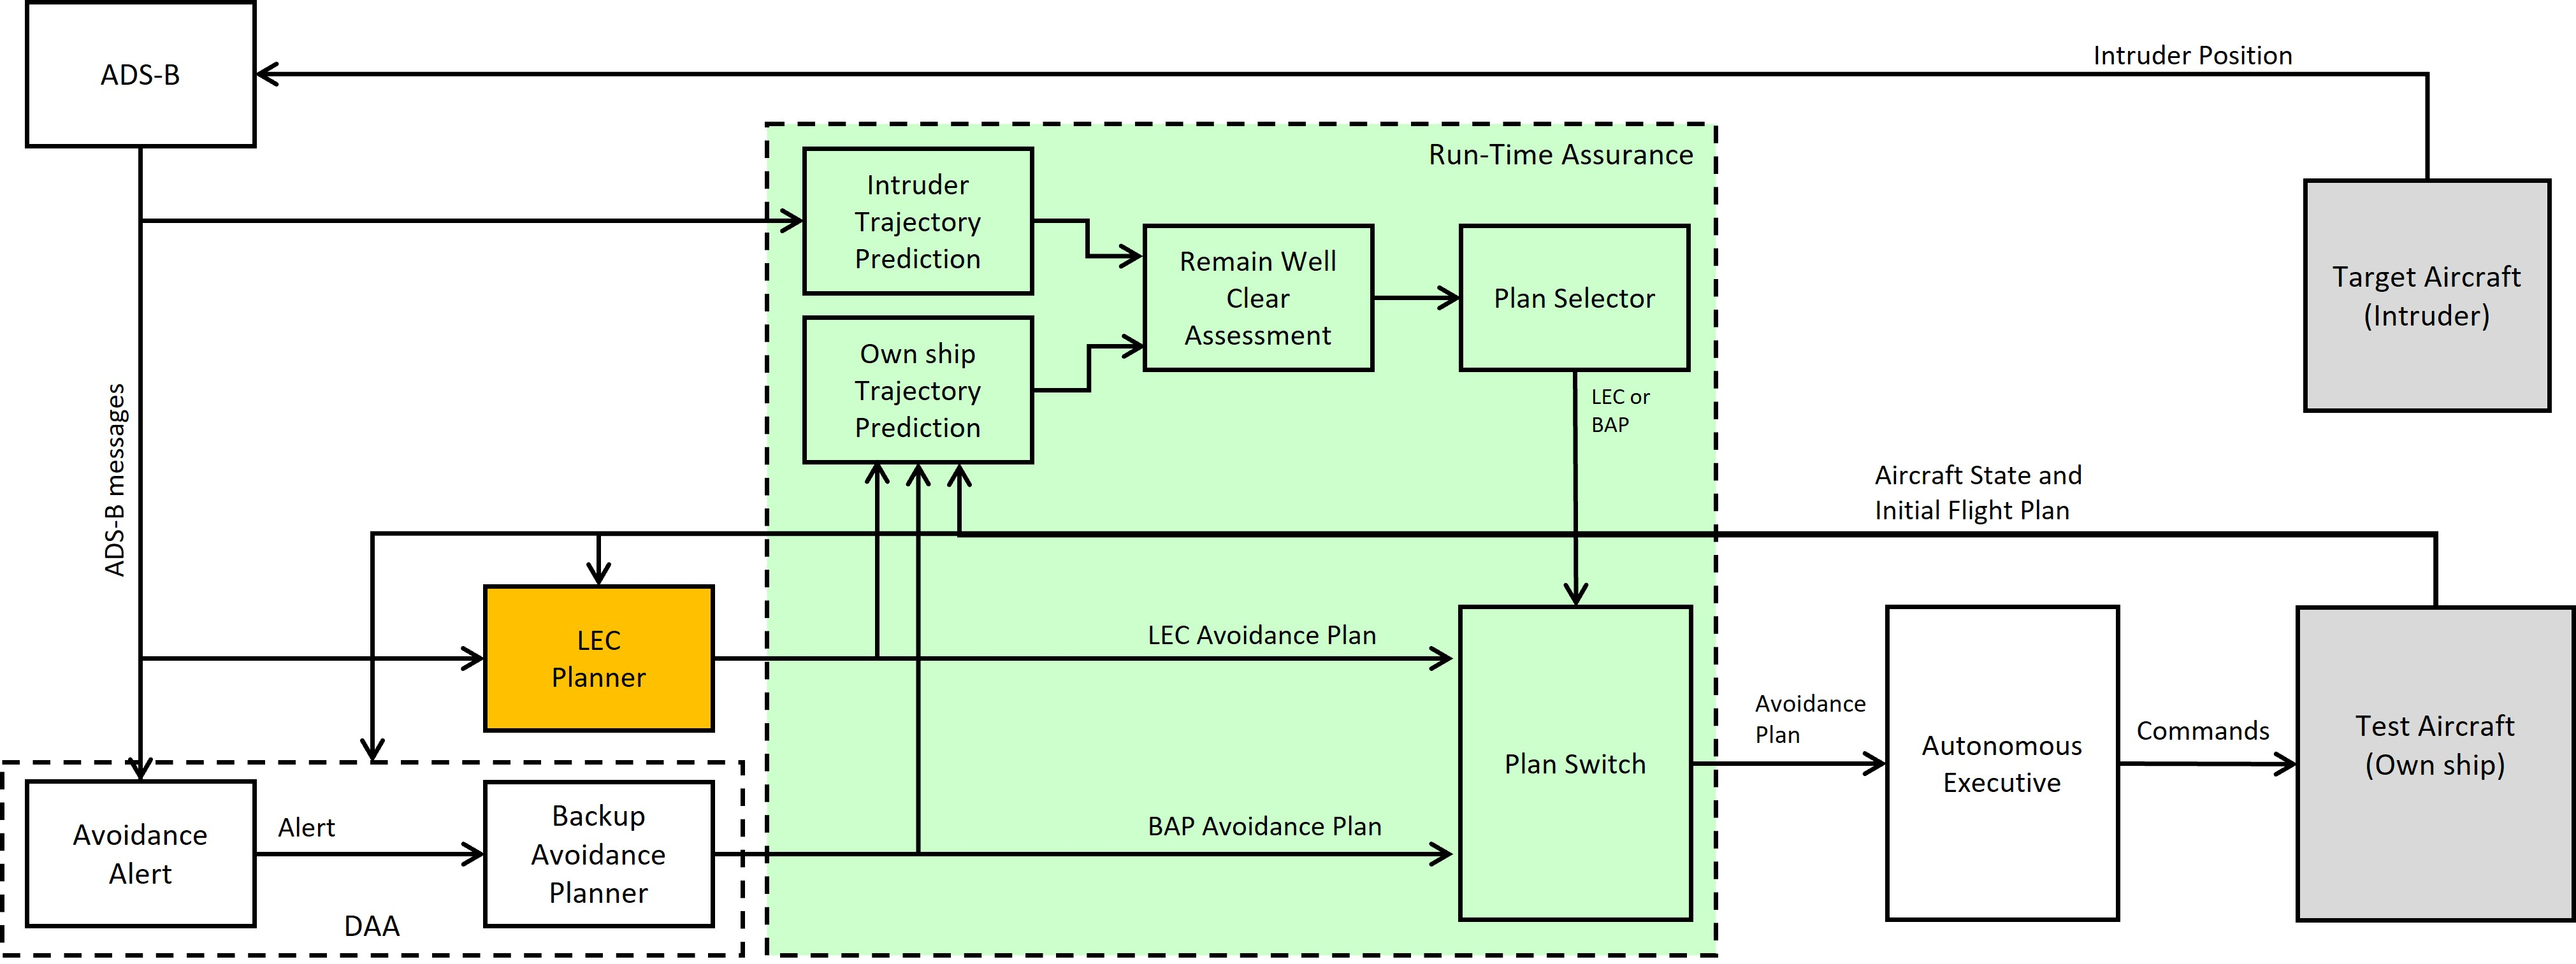
\includegraphics[width=\textwidth]{figures/rta-arch.jpg}
	\caption{Run-Time Assurance Architecture}
	\label{fig:rta-arch}
\end{figure*}

\subsection{Trajectory prediction} 
Trajectory prediction over a defined prediction horizon (in time units) consists of prediction of both the intruder and own-ship trajectories based on underlying assumptions of the intruder's future velocity and the own-ship's ability to track the avoidance flight plans from the LEC and the Safe Backup Planner. For the application in consideration, the prediction horizon was set to 180 seconds under the assumption that the avoidance flight plans produced would be frozen for this time period. In cases where the avoidance plans can be generated more frequently, the prediction horizon can appropriately be reduced which should improve the accuracy of intruder trajectory prediction and allow for more confidence in the SWC evaluation.

For the intruder, each incoming ADS-B message is processed as a measurement to a tracking filter designed as per Appendix D in \cite{DO_366A}. The tracking filter assumes that the intruder aircraft is either in a constant velocity (CV) mode or in a constant speed turn (CT) mode. The multiple-model tracking filter is designed to be robust to basic errors in the ADS-B message data (such as data with too small or large uncertainties), missing data or repeat data, but mostly the ADS-B data is considered a trustworthy source of information of the intruder 3D position. The tracking filter produces estimates of the intruder current position and velocity along with their respective uncertainties, and with a prediction of the specific mode of the intruder behavior (CV/CT). The trajectory prediction propagates the estimate from the tracking filter forward in time by assuming the aircraft continues in its current mode (CV/CT) with a growth model in the longitudinal velocity uncertainty and a cross-track position uncertainty, with the cross-track position uncertainty capped to a maximum value. The uncertainties in the intruder trajectories can be visualized as ellipses whose semi-major/semi-minor axes are aligned with the longitudinal/normal to velocity vector and whose lengths are proportional to the uncertainties along/normal to the velocity vector. These assumptions allow to account for decaying confidence over longer prediction horizons.

The own-ship trajectory predictions along the avoidance flight plans assume a kinematic model of the own-ship behavior using performance parameters such as maximum bank angle, roll-rate, longitudinal acceleration, etc. The trajectory prediction assumes that the first waypoint of the avoidance flight plans lies directly in the path of the current velocity vector. The own-ship trajectory consists of constant ground speed segments between waypoints and constant speed arcs connecting line segments between consecutive waypoints. As the actual aircraft is flying constant airspeed, and not ground speed, deviations between the predicted and actual aircraft trajectories are expected. These deviations are accounted for by a fixed tracking error bound that is configurable. The tracking error bound $+$ vehicle size parameter are padded onto the specified SWC separation distance to produce a conflict radius threshold around the own-aircraft.

The trajectory prediction models are run internally at a high-rate ($>= $ 10 Hz) for both the intruder and own-ship, but the output trajectories are sampled at 1 Hz to produce time-stamped discretized trajectory points which are evaluated for conflicts as discussed in the next sub-section.

\subsection{SWC assessment} 
The SWC assessment consists of evaluating time-stamped samples of the predicted trajectory of the intruder and the own-aircraft trajectory along each produced avoidance flight plan. The evaluation considers the intersection of the uncertainty ellipse around an intruder predicted trajectory sample with the conflict circle around the corresponding own-aircraft predicted trajectory sample. The probability of intersection is determined using the analytical approximations documented in Section IV of \cite{prob_conflict_detection}. If the probability exceeds a configurable threshold, then the flight plan is determined to be unsafe. 

In addition to the boolean determination of safety, the point to closest approach (CPA) between the own-ship and intruder predicted trajectories is calculated along with the time to CPA. The CPA metrics allow the Decision Logic Component to choose between plans that are both marked unsafe by the SWC assessment. These metrics allow for a comparison with the actual measured CPA metrics during simulation and test flights as a way to evaluate the run-time monitor performance.